\chapter{Opis projektnog zadatka}
		
		\textbf{\textit{dio 1. revizije}}\\
		
		Aplikacija ByteBit inovativno je rješenje namijenjeno provjeri 
		programerskih vještina, omogućavajući korisnicima sudjelovanje u 
		programskim natjecanjima i vježbanje rješavanja zadataka. Aplikacija 
		se može implementirati kao web ili desktop platforma koristeći 
		objektno-orijentirane programerske jezike, sa podrškom za kompilaciju
		i evaluaciju rješenja u najmanje jednom programskom jeziku.\\

		Glavne funkcionalnosti aplikacije uključuju:
		\begin{packed_item}
    	\item \textbf{Pregledavanje zadataka i kalendar natjecanja:} 
		Korisnici mogu pregledavati dostupne zadatke i kalendar natjecanja, 
		što omogućava planiranje sudjelovanja i pripremu.
    	\item \textbf{Profili korisnika:} Natjecatelji imaju profile s 
		prikazom statistika njihovih rezultata, uključujući broj točno 
		riješenih i isprobanih zadataka, kao i pehare za osvojena natjecanja.
		Profili voditelja sadrže informacije o učitanim zadacima i 
		organiziranim natjecanjima.
 		\item \textbf{Registracija korisnika:} Registracija zahtijeva 
		osnovne podatke kao što su korisničko ime, fotografija, lozinka, 
		ime, prezime i email adresa. Administrator potvrđuje registraciju,
		a u slučaju voditelja natjecanja potrebna je i dodatna verifikacija.
    	\item \textbf{Natjecanja:} Početkom natjecanja, zadaci postaju 
		vidljivi aktivnim natjecateljima. Nakon završetka, zadaci su
		dostupni svima. Postoji mogućnost slanja datoteka s programskim
		kodom i objavljivanje rang lista po bodovima, uzimajući u
		obzir vrijeme i točnost rješenja.
    	\item \textbf{Prikaz rješenja:} Natjecatelji mogu vidjeti 
		rješenja drugih natjecatelja nakon natjecanja, dok su tijekom 
		natjecanja vidljiva samo ako su sami točno riješili zadatak.
    	\item \textbf{Vježbanje:} Natjecatelji mogu vježbati zadatake i 
		učitavati rješenja, s automatskom provjerom točnosti i vremenskih ograničenja.
   		\item \textbf{Virtualna natjecanja:} Natjecatelji mogu stvoriti 
		vlastita virtualna natjecanja odabirom prošlih natjecanja ili 
		nasumičnim odabirom zadataka, a rezultati se uspoređuju s originalnim.
    	\item \textbf{Uloga voditelja:} Voditelji imaju mogućnost učitavanja 
		novih zadataka, organiziranja natjecanja, i odabira zadataka koji će 
		biti aktivni tijekom natjecanja, uz mogućnost uređivanja vlastitih zadataka.
   		\item \textbf{Administrativne funkcije:} Administratori imaju ovlasti 
		za upravljanje korisničkim računima i uređivanjem svih zadataka i 
		natjecanja, bez mijenjanja prethodno ostvarenih rezultata.\\
		\end{packed_item}


		Trenutno postoje brojne platforme poput Codeforces, LeetCode,
		HackerRank i drugih koje nude slične funkcionalnosti. Razlike
		u odnosu na BytePit bi se mogle ogledati u specifičnostima kao
		što su lokalizacija (jezik i regionalni fokus), specijalizacija
		za određene programerske jezike ili tehnologije, ili u razini
		personalizacije korisničkog iskustva.
		Slična rješenja i razlike:
		\begin{packed_item}
			\item \textbf{Codeforces}: Fokusira se na konkurentno programiranje s
			redovitim natjecanjima. BytePit bi mogao uključivati više edukativnih
			resursa i prilagodljiva virtualna natjecanja.
			\item \textbf{LeetCode}: Specijaliziran za pripremu tehničkih intervjua.
			BytePit može nuditi širi raspon zadatka, uključujući one van konteksta intervjua.
			\item \textbf{HackerRank}: Osim izazova u programiranju, nudi i podršku
			za tvrtke u regrutiranju. BytePit bi mogao dodati vrednost kroz specifične
			profile natjecanja i detaljnu statistiku.Sličan koncept, ali s fokusom na
			poslovne korisnike. BytePit bi mogao biti više usmjeren na edukaciju i natjecanja.\\
		\end{packed_item}


		BytePit bi mogao privući širok spektar korisnika, od početnika u programiranju 
		koji traže mjesto za učenje i prakticiranje, do iskusnih programera koji žele 
		oštriti svoje vještine ili sudjelovati u natjecanjima, te edukativnih institucija 
		koje traže platformu za organiziranje natjecanja ili kao alat u nastavi. Ova 
		raznolikost korisnika stvara dinamično okruženje u kojem se znanje i iskustvo 
		neprestano razmjenjuju, pružajući beskrajne mogućnosti za učenje i napredak. 
		S jedne strane, početnici imaju priliku učiti kroz praksu, rješavajući stvarne 
		probleme i dobivajući povratne informacije od iskusnijih kolega. S druge strane, 
		iskusni programeri mogu se suočavati s izazovnijim problemima i sudjelovati u 
		zahtjevnijim natjecanjima, što ih stavlja u poziciju mentora, potičući ih na 
		daljnji razvoj i dijeljenje znanja. Edukativne institucije mogu koristiti BytePit 
		za stvaranje prilagođenih tečajeva i kurikuluma, pružajući studentima praktično 
		iskustvo koje je ključno za njihov razvoj. Poslodavci koji traže talentirane 
		programere mogli bi koristiti platformu za identifikaciju potencijalnih kandidata, 
		provodeći natjecanja ili izazove koji služe kao dio procesa zapošljavanja ili kroz 
		analizu rješenja i pristupa problemima koje programeri koriste na platformi.
		\\

		BytePit bi trebao biti projektiran s mogućnostima prilagodbe, što bi uključivalo 
		konfigurabilne module za natjecanja, personalizirane profile korisnika, i fleksibilan 
		sustav ocjenjivanja. Prilagodba omogućava korisnicima da kreiraju jedinstveno 
		iskustvo koje odgovara njihovim specifičnim potrebama i stilu učenja ili rada. 
		Personalizirani profili omogućavaju korisnicima da predstave svoje vještine i 
		postignuća, kao i da prate svoj napredak kroz različite metrike i statistike. 
		Fleksibilan sustav ocjenjivanja omogućava različite forme evaluacije, od standardnog 
		bodovanja do složenih algoritama koji mogu vrednovati efikasnost koda ili kreativno 
		rješavanje problema. Ovo omogućava platformi da raste i evoluira zajedno sa svojim 
		korisničkim bazama i tehnološkim trendovima, ostajući relevantna i privlačna za 
		široki spektar korisnika, od individualaca i obrazovnih institucija do korporacija 
		i tehničkih zajednica.
		\\

		Opseg projekta uključuje dizajniranje i implementaciju korisničkih sučelja, koje 
		moraju biti intuitivna i pristupačna, osiguravajući ugodno iskustvo za sve korisnike, 
		neovisno o njihovom tehničkom znanju ili iskustvu u programiranju. Back-end servisi 
		za upravljanje bazom podataka moraju biti robustni i optimizirani za brzu obradu 
		upita, što je ključno za održavanje visoke performanse platforme čak i pod velikim 
		opterećenjem. Sustav za evaluaciju koda mora biti precizan i pouzdan, sposoban za 
		brzo i efikasno procjenjivanje raznovrsnih programskih rješenja koja korisnici 
		predaju. Sustav za autentifikaciju i autorizaciju korisnika treba osigurati da su 
		svi podaci sigurni i da pristup platformi
		\\

		Nadogradnje projekta mogu uključivati:
		\begin{packed_item}
			\item Integraciju s vanjskim servisima poput GitHub-a za uvoz postojećeg koda.
			\item Implementaciju naprednijih algoritama za detekciju plagijata.
			\item Proširenje podrške za više programskih jezika i tehnoloških okvira.
			\item Razvoj mobilne aplikacije za pristup platformi.
			\item Uvođenje umjetne inteligencije za personalizirane preporuke zadataka
			na temelju korisnikovih prethodnih aktivnosti i uspjeha.
			\item "Gamification" sustav za nagrađivanje korisnika za postignuća i napredak.
		\end{packed_item}


		\eject
		
		\section{Primjeri u \LaTeX u}
		
		\textit{Ovo potpoglavlje izbrisati.}\\

		U nastavku se nalaze različiti primjeri kako koristiti osnovne funkcionalnosti \LaTeX a koje su potrebne za izradu dokumentacije. Za dodatnu pomoć obratiti se asistentu na projektu ili potražiti upute na sljedećim web sjedištima:
		\begin{itemize}
			\item Upute za izradu diplomskog rada u \LaTeX u - \url{https://www.fer.unizg.hr/_download/repository/LaTeX-upute.pdf}
			\item \LaTeX\ projekt - \url{https://www.latex-project.org/help/}
			\item StackExchange za Tex - \url{https://tex.stackexchange.com/}\\
		
		\end{itemize} 	


		
		\noindent \underbar{podcrtani tekst}, \textbf{podebljani tekst}, 	\textit{nagnuti tekst}\\
		\noindent \normalsize primjer \large primjer \Large primjer \LARGE {primjer} \huge {primjer} \Huge primjer \normalsize
				
		\begin{packed_item}
			
			\item  primjer
			\item  primjer
			\item  primjer
			\item[] \begin{packed_enum}
				\item primjer
				\item[] \begin{packed_enum}
					\item[1.a] primjer
					\item[b] primjer
				\end{packed_enum}
				\item primjer
			\end{packed_enum}
			
		\end{packed_item}
		
		\noindent primjer url-a: \url{https://www.fer.unizg.hr/predmet/proinz/projekt}
		
		\noindent posebni znakovi: \# \$ \% \& \{ \} \_ 
		$|$ $<$ $>$ 
		\^{} 
		\~{} 
		$\backslash$ 
		
		
		\begin{longtblr}[
			label=none,
			entry=none
			]{
				width = \textwidth,
				colspec={|X[8,l]|X[8, l]|X[16, l]|}, 
				rowhead = 1,
			} %definicija širine tablice, širine stupaca, poravnanje i broja redaka naslova tablice
			\hline \SetCell[c=3]{c}{\textbf{naslov unutar tablice}}	 \\ \hline[3pt]
			\SetCell{LightGreen}IDKorisnik & INT	&  	Lorem ipsum dolor sit amet, consectetur adipiscing elit, sed do eiusmod  	\\ \hline
			korisnickoIme	& VARCHAR &   	\\ \hline 
			email & VARCHAR &   \\ \hline 
			ime & VARCHAR	&  		\\ \hline 
			\SetCell{LightBlue} primjer	& VARCHAR &   	\\ \hline 
		\end{longtblr}
		

		\begin{longtblr}[
				caption = {Naslov s referencom izvan tablice},
				entry = {Short Caption},
			]{
				width = \textwidth, 
				colspec = {|X[8,l]|X[8,l]|X[16,l]|}, 
				rowhead = 1,
			}
			\hline
			\SetCell{LightGreen}IDKorisnik & INT	&  	Lorem ipsum dolor sit amet, consectetur adipiscing elit, sed do eiusmod  	\\ \hline
			korisnickoIme	& VARCHAR &   	\\ \hline 
			email & VARCHAR &   \\ \hline 
			ime & VARCHAR	&  		\\ \hline 
			\SetCell{LightBlue} primjer	& VARCHAR &   	\\ \hline 
		\end{longtblr}
	


		
		
		%unos slike
		\begin{figure}[H]
			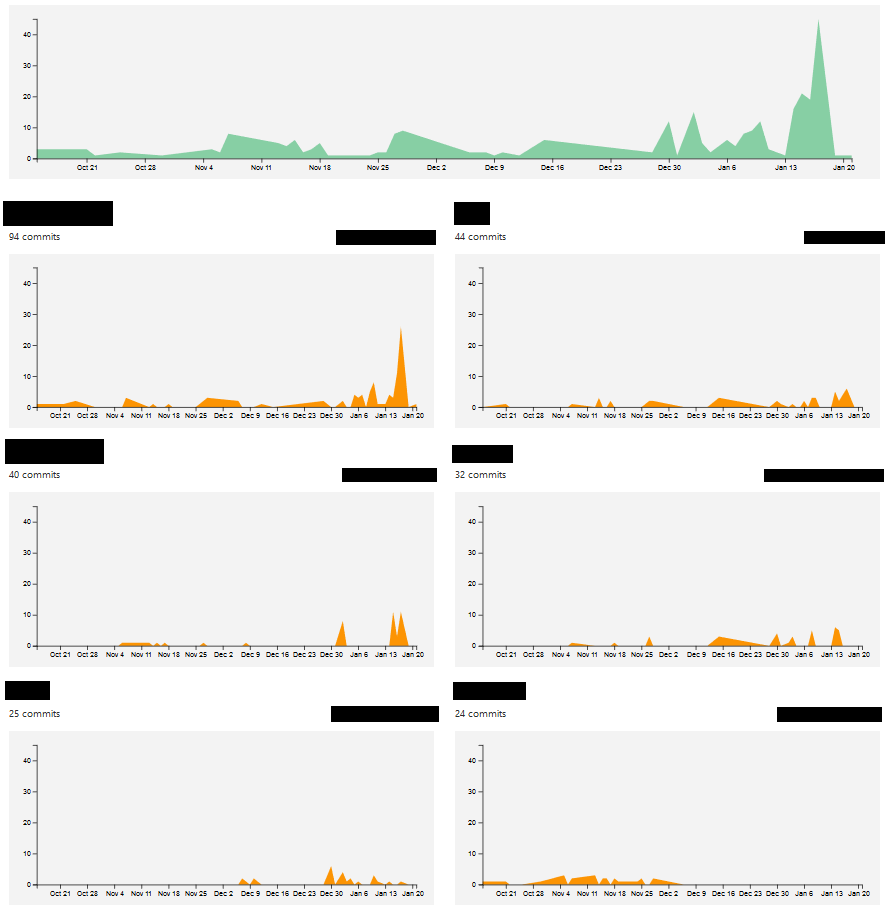
\includegraphics[scale=0.4]{slike/aktivnost.PNG} %veličina slike u odnosu na originalnu datoteku i pozicija slike
			\centering
			\caption{Primjer slike s potpisom}
			\label{fig:promjene}
		\end{figure}
		
		\begin{figure}[H]
			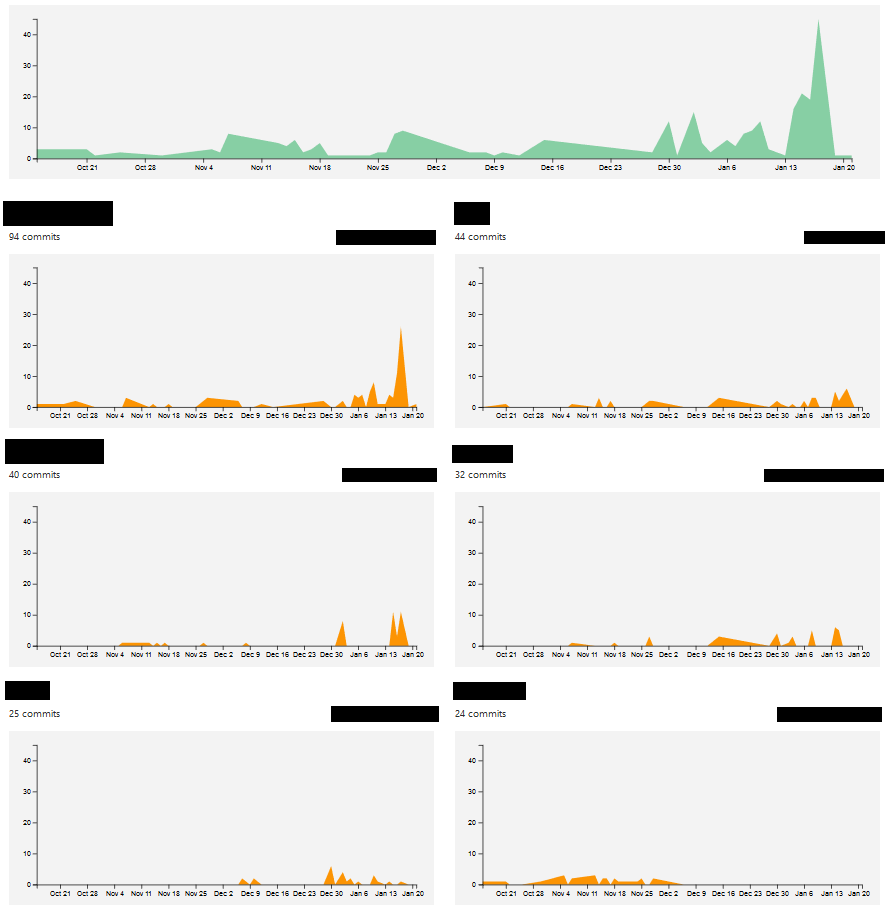
\includegraphics[width=\textwidth]{slike/aktivnost.PNG} %veličina u odnosu na širinu linije
			\caption{Primjer slike s potpisom 2}
			\label{fig:promjene2} %label mora biti drugaciji za svaku sliku
		\end{figure}
		
		Referenciranje slike \ref{fig:promjene2} u tekstu.
		
		\eject
		
	